\section{Reaching}
\label{sec:reaching}

In this section, we describe two approaches which have been 
implemented on our robot to solve the reaching task. A first method 
uses the forward mapping between the arm joint space and the three 
dimensional position of the hand represented in the head reference 
frame $\begin{bmatrix} \theta_y & \theta_p & \alpha_v^d\end{bmatrix}^\top 
\in \mathbb R^3$. 
The second method uses a visual servoing technique to control the 
speed of the arm so to minimize the position of the hand in the 
image plane with respect to a desired target (usually the fixated object).

\subsection{Open Loop Reaching}
%
Suppose the robot is tracking a target using the control strategy described in 
Section \ref{Sec:TrackerController}. In the further assumption of perfect 
tracking (the visual error is zero), the three dimensional spatial position 
of the target with respect to the robot, denoted $\tilde {\mathbf x}_{target} 
\in \mathbb R^3$, 
is a function of the head configuration $\mathbf q_{head} =
\begin{bmatrix} \theta_y & \theta_p & \theta_r & \alpha_v^d & \alpha_v^c & \alpha_t^c \end{bmatrix}^\top \in \mathbb R^6$.
However, the representation of the target position, $\tilde {\mathbf x}_{target}$, 
in terms of the full head configuration, $\mathbf q_{head}$, is clearly redundant.
Specifically, the same target position can be represented different head configurations. 
In order to obtain a one to one mapping between the target configuration and the 
head position we have to carefully analyze the {\tt tracker controller}. During tracking 
$\theta_r$ is maintained stationary ($\theta_r^d = 0$), while the head controller 
poses additional constraints on the head joints; in particular we know from section 
\ref{Sec:TrackerController} that the controller minimizes $\alpha_t^c$ and
$\alpha^c_v$ (see equation (\ref{Eq:HeadEyeControl})) so that they asymptotically
converge to $\alpha_t^c \rightarrow 0$ and $\alpha_v^c \rightarrow 0$. Ideally, after 
fixation has been achieved, we should have:
%
\begin{eqnarray}
{\mathbf q}_{head}=
\begin{bmatrix} \theta_y & \theta_p & 0 & \alpha_v^d & 0 & 0 \end{bmatrix}^\top \in \mathbb R^6.
\end{eqnarray}
%
Since there exists a one to one mapping between the three dimensional position of the target 
$\tilde {\mathbf x}_{target}$ and the three non-zero variables $\theta_y$, $\theta_p$ 
and $\alpha_v^d$, we can define:
%
\begin{eqnarray}
\mathbf x_{target}=
\begin{bmatrix} \theta_y & \theta_p & \alpha_v^d\end{bmatrix}^\top \in \mathbb R^3.
\end{eqnarray}
%
This new variable $\mathbf x_{target} \in \mathbb R^3$ uniquely codes the position 
of the target. The representation is very similar to a three dimensional polar 
representation in which $\theta_y$ and $\theta_p$ code respectively azimuth 
and elevation, while distance is substituted with $\alpha_v$ (\emph{vergence} angle). 

If the robot is tracking the hand, the same subset of the head joint space can be used to code the spatial location of the hand:
%
\begin{eqnarray*}
\xhand=
\begin{bmatrix} \theta_y & \theta_p & \alpha_v^d\end{bmatrix}^\top \in \mathbb R^3.
\end{eqnarray*}
%
Under these assumptions we can train a neural network to approximate the 
forward mapping between the arm joint space $\qarm$ and the 
position of the hand $\xhand$:
%
\begin{equation} 
\label{Eq:forward}
\mathbf x_{hand}=f_{arm}(\mathbf q_{arm}), \qquad f_{arm} : \mathbb R^3 \longrightarrow \mathbb R^4.\end{equation}
%
Suppose now that we want to control the robot to reach for a target 
that is currently fixated. Formally the problem can be formulated 
as determining the value of $\qarm$ which solves the 
following minimization:
%
\begin{equation} 
\label{Eq:reaching1}
  \displaystyle\min_{\qarm} \left(J\right)=\displaystyle\min_{\qarm}
  \left\|\mathbf x_{hand} - \mathbf x_{target}\right\|^2,
\end{equation}
%
where $\mathbf x_{target}$ is measured from the encoders of the head, while 
$\mathbf x_{hand}$ is computed from $\qarm$ through Eq. (\ref{Eq:forward}). 
Given the redundancy of the arm kinematics the minimization 
(\ref{Eq:reaching1}) has infinite solutions. To 
overcome this problem we constrained the solution so that one of the joint, 
for example joint number 2, is forced to remain as close as possible to 
a predefined position $q_{20}$:
%
\begin{equation} 
\label{Eq:reaching2}
  \displaystyle\min_{\qarm}\left(J_c\right)=\displaystyle\min_{\qarm}
  \left[
  \left\|\mathbf x_{hand} - \mathbf x_{target}\right\|^2 + \left(q_{arm,2}-q_{20}\right)^2
  \right].
\end{equation}

The optimization of (\ref{Eq:reaching2}) can be performed numercially with 
different tools. Discussing the different properties of these numerical 
tools falls outside the scope of this paper. In our implementation, we used 
the downhill simplex method \cite{ne:Computer:65} as implemented in 
\cite{mo:Press:90}.

\subsection{Learning the open loop reaching}
\label{sec:learning-open-loop}
%
To learn the forward map of Eq. (\ref{Eq:forward}) we programmed 
the robot to perform random movements with the arm (chosen to uniformly sample 
a predefined region in the robot workspace). During this ``exploratory'' 
phase the robot tracked the hand, and collected samples of the form:
%
\begin{center}
\begin{math}
  \left(\begin{array}{cc}
    \qarm^i , \xhand^i\end{array}\right)_{i \in 0,1\dots}
\end{math}
\end{center}
%
A neural network was then trained to learn the relation:
%
\begin{equation} 
  \xhand=\hat{f}_{arm}\left(\qarm \right),
\end{equation}
%
which approximates Eq. (\ref{Eq:forward}).

In the experiment reported in this paper we collected a data set of 
about 2890 samples that we devided in a training set (2168 samples) and 
a test set (725 samples). We used the training set to train a neural 
network to approximate Eq. (\ref{Eq:forward}). The neural network 
we employed was the Receptive Field Weighted Regression model proposed 
by \cite{schaal98Constructive}. This network implements an online learning
method, meaning that a learning step is performed every time a new 
sample is shown to the network. All samples in the training set were shown
to the network only once in a random order. After each training step the 
performance of the network was validated on the whole test set, by computing
the mean squared error between each sample in the test set and the 
corresponding network output. The plot in figure (\ref{fig:reaching-error})
shows the trend of the error on the test set during learning. The final 
average error was 1.89 degrees with standard deviation 1.49.

In the experiment reported in this paper learning was performed offline. 
This was to simplify the analysis of the results and perform cross-validation 
on a predefined test set. However, the learning algorithm we used was purely 
incremental (each sample was shown to the network only once and immediatly 
discarded), so from a point of view of the learning it would be 
straightforward to have an online implementation of the same mechanism.

\begin{figure}[tbp]
\label{fig:reaching-error}
\centerline{
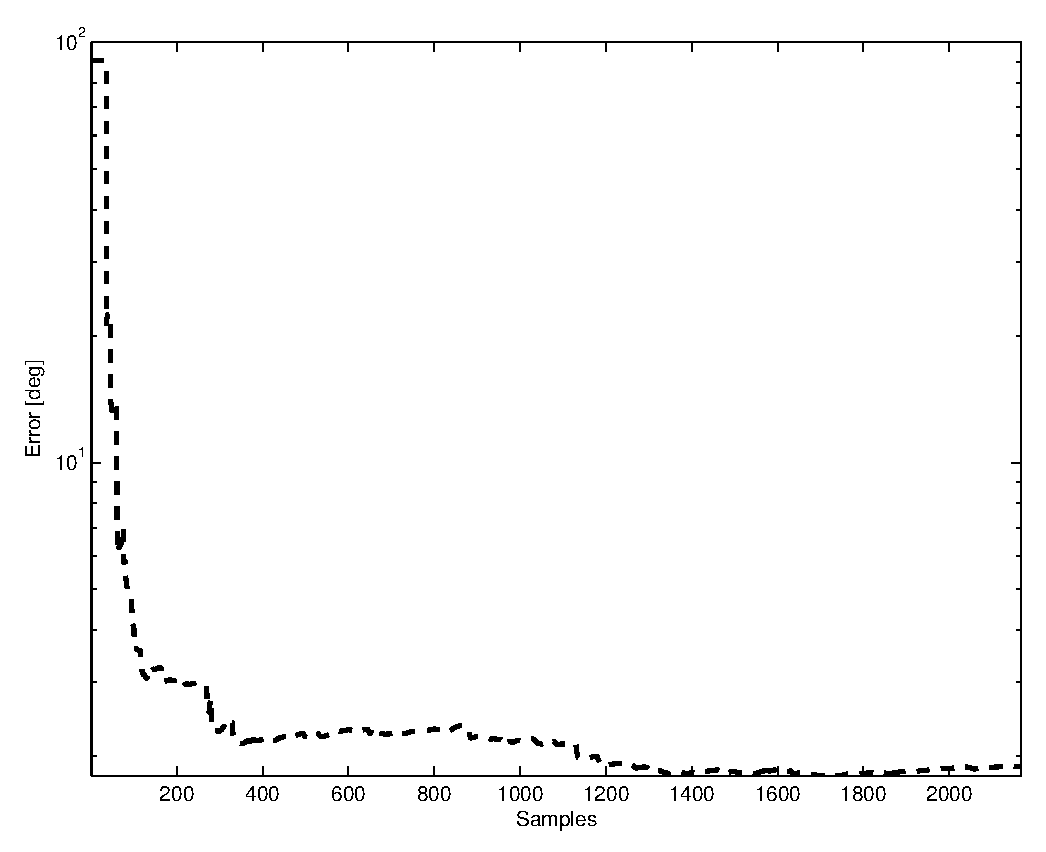
\includegraphics[width=4.0in, angle=0 ]{./Figure/reachingError1.eps}
} \caption{Error} 
\end{figure}

\subsection{Closed Loop Reaching}
%
Under the assumption that the robot can visually measure the distance
between the hand and the target, we can implement a closed loop 
control to reach for a visually identified target.

We know that the Jacobian matrix relates movement of the arm 
$\deltaqarm$ in the joint space with displacement of the hand 
\begin{math}\deltauhand=
\left[ \begin{array}{ccc}
  \delta u_r & \delta v_r & \delta u_{lm}
\end{array} \right]^T\end{math} 
in the image plane, formally:
%
\begin{equation} 
\label{eq:jacobian1}
  \deltauhand=
  \tilde{\mathbf J}\left(\mathbf q_{arm}, \mathbf q_{head}\right)
  \deltaqarm,
\end{equation}
%
where $\tilde{\jacobian} \in \mathbb R^{3 \times 4}$ depends on 
both the configuration of the arm and the head. Due to the 
additional constrained posed by the head tracker, we showed
that only a subset of $\qhead$, $\xtarget$, is 
sufficient to uniquely identify the position of the head, so we 
can rewrite equation (\ref{eq:jacobian1}) as:
%
\begin{equation}
\label{eq:jacobian2}
  \deltauhand=
  \tilde{\jacobian}\left(\qarm, \xtarget\right)
  \deltaqarm, \qquad \tilde{\jacobian} \in \mathbb R^{3,4}.
\end{equation}
%

From equation (\ref{Eq:forward}) it is clear that 
$\qarm$ and $\xtarget$ are redundant and only $\qarm$ is 
sufficient to uniquely identify the position of the head. Eq.
(\ref{eq:jacobian2}) can be further simplified to:
%
\begin{equation} 
\label{eq:jacobian3}
  \deltauhand=
  \jacobian \left(\qarm\right)
  \deltaqarm,\qquad \jacobian \in \mathbb R^{3,4}
\end{equation}
%
in which $\jacobian$ depend only on the arm 
joint configuration $\qarm$.

Suppose now the robot has to reach for an object, whose visual position is 
represented by $\utarget$. To solve the problem 
the controller of the arm needs to compute the arm command which minimizes 
the error:
%
\begin{equation}
  e=\left||\uhand-\utarget\right||^2.
\end{equation}
%
When the head tracker has achieved convergence on the object, 
$\utarget \approx 0 $ and $e$ $\approx \left||\uhand\right||^2$.
The following control strategy minimizes $e$:
%
\begin{equation}
\mathbf{\dot q}_{arm}=-k \cdot \jacobian^\# \uhand, 
\qquad \jacobian^\# \in \mathbb R^{4,3},
\end{equation}
%
where $\jacobian^\#$ is the pseudo-inverse of $\jacobian$.

\subsection{Learning the Arm Jacobian}
%
In the previous section we used the Jacobian of the manipulator
$\jacobian$ (actually its pseudo-inverse $\jacobian^\#$) to 
control the arm to reach for a visually identified object. In 
this section we describe a procedure by which the robot can 
autonomously acquire $\jacobian$ and $\jacobian^\#$.

As described in Section \ref{sec:learning-open-loop}, the robot 
moves the arm randomly, while maintainining gaze on the hand. At 
the end of each movement $j$ the arm is in a configuration 
$\qarm^j$,  while the eyes are fixating the hand 
($\uhand \approx 0$) with the gaze centered within the neck 
(convergence of the head tracker has been achieved). Each 
arm configuration corresponds to a different value of 
$\jacobian_j=\jacobian\left(\qarm^j\right)$. 
Now the robot inhibits the head tracker and performs a sequence $m$
of small arm movements $\deltaqarm^k$ which perturb 
$\uhand$ of small amounts $\deltauhand^k$:
%
\begin{center}
\begin{math}
  \left(\begin{array}{cc}
    \deltauhand^k , 
	\deltaqarm^k \end{array}
  \right)_{k \in 0,1\dots,m}
\end{math}
\end{center}
%
All $m$ perturbations $\deltauhand^k$ and 
$\deltaqarm^k$ are linearly realated thourgh $\jacobian_i$ 
as described in Eq. (\ref{eq:jacobian2}). From these $m$ 
observations we can derive a least squares estimation of $\jacobian_j$ from 
which, in turn, we can compute the pseudo-inverse $\jacobian_j^\#$. 
Re-iterating this procedure leads to the collection of a series of examples:
%
\begin{center}
\begin{math}
  \left(\begin{array}{cc}
    \qarm^j , \jacobian_j^\# \end{array}\right)_{j \in 0,1\dots}
\end{math}
\end{center}
%
An approximation $\hat{\jacobian}^\#$ of $\jacobian^\#$ is finally
obtained by training a neural network:
%
\begin{equation}
\mathbf{g}\left(\qarm\right), \qquad g : \mathbb R^4 \longrightarrow \mathbb R^{12},
\end{equation}
%
whose output components are the coefficients of 
$\hat{\jacobian}^\# \in \mathbb R^{4 \times 3}$.
%

